% Charlotte Geiger - Manuel Lippert - Leonard Schatt
% Physikalisches Praktikum

% 3.Kapitel  Protokoll

% Variables
\def\skalierung{0.65}

\chapter{Messprotokoll}
\label{chap:protokoll}

Das Messprotokoll wurde am Versuchstag handschriftlich erstellt und hier als
PDF-Datei eingefügt. 

\section*{Zusatz}
Zusätzlich fügen wir die Bilder und die verwendeten Schaltungen des Versuchs nch dem Protokoll an zur besseren Übersicht.

% Einbindung des Protokolls als pdf (mit Seitenzahl etc.)
% Erste Seite mit Überschrift
%\includepdf[pages = 1, landscape = false, nup = 1x1, scale = \skalierung , pagecommand={\thispagestyle{empty}\chapter{Protokoll}}]
%            {03-Protokoll/Protokoll.pdf}
% Restliche Seiten richtig skaliert
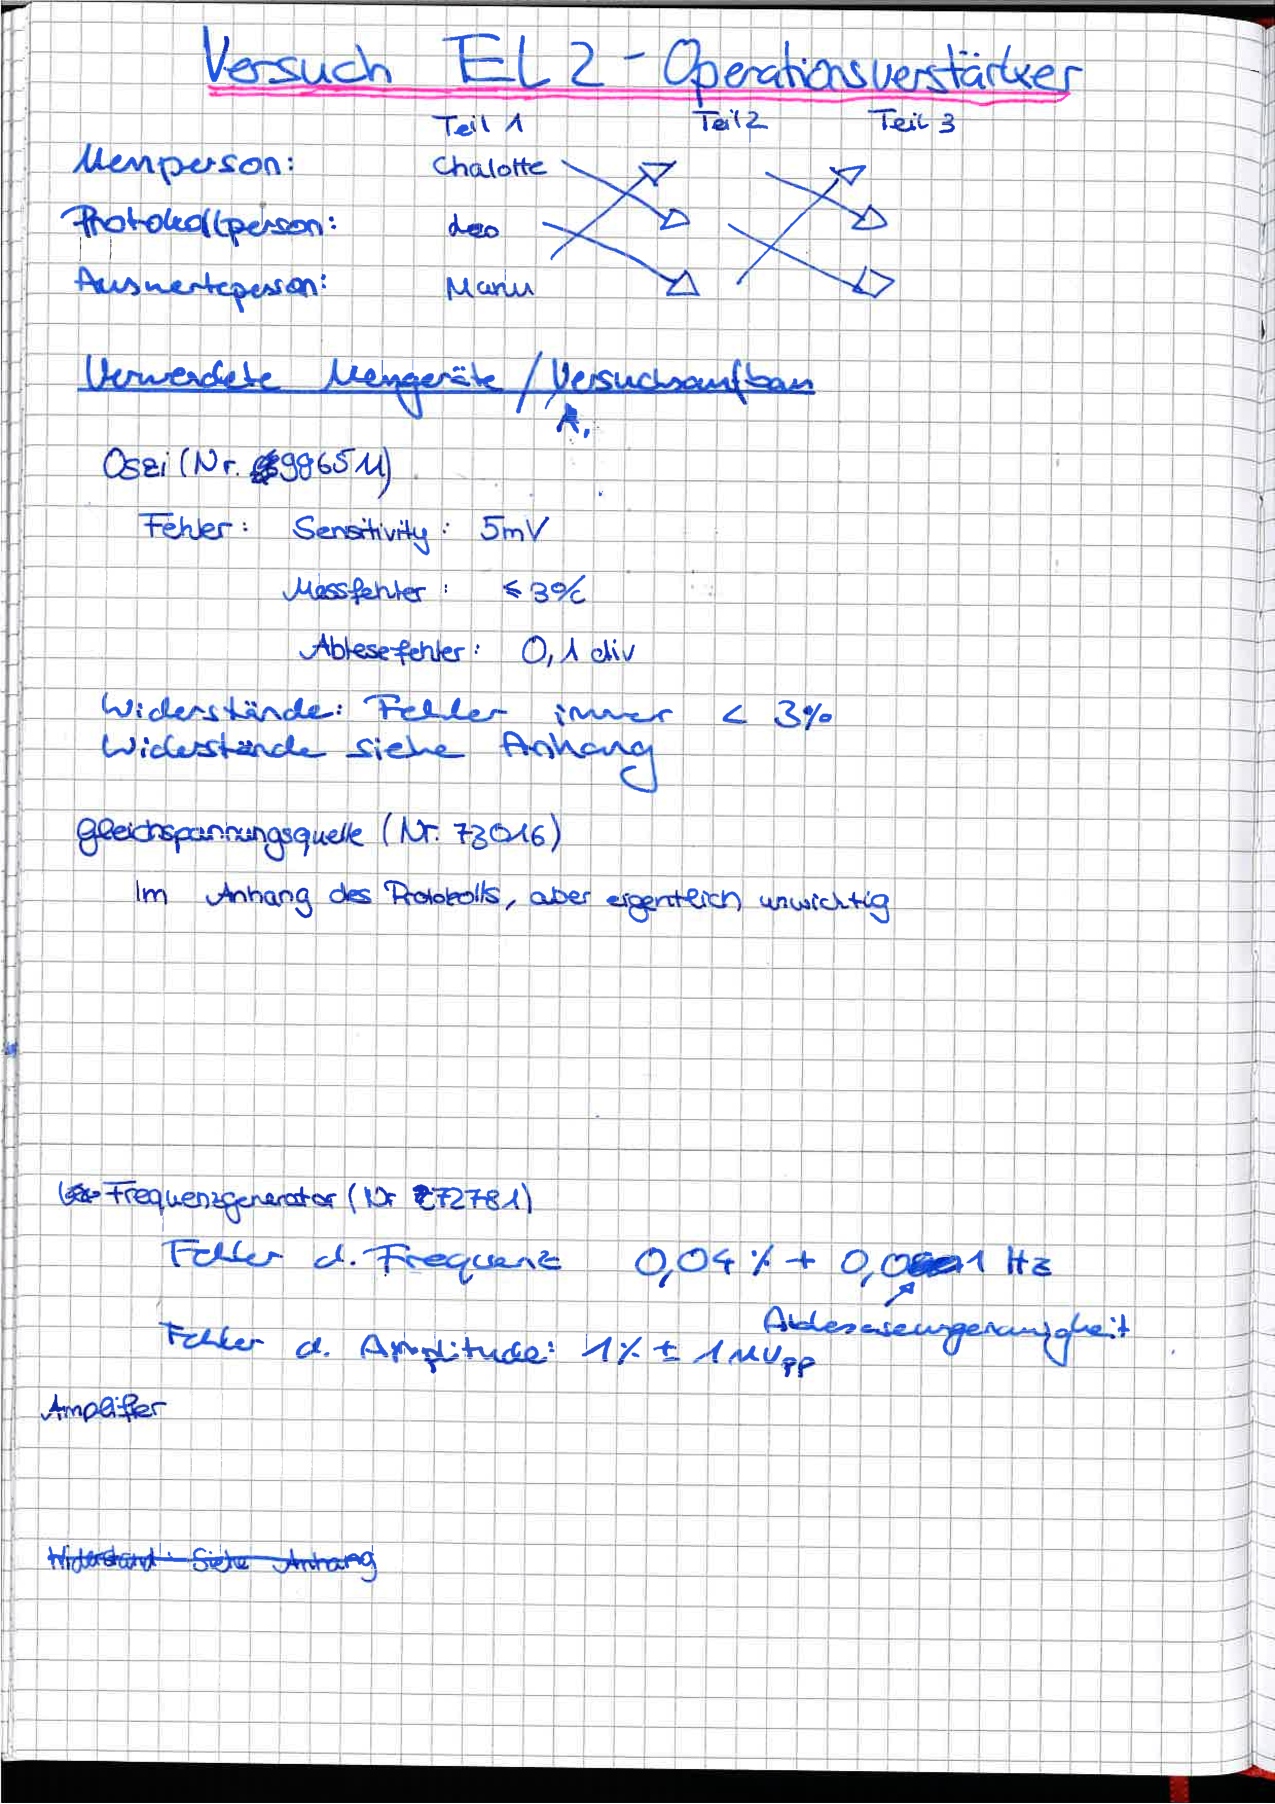
\includepdf[pages = -, landscape = false, nup = 1x1, scale = \skalierung , pagecommand={}]{30-ProtokollEL2.pdf}

%\section*{Steckbretter}
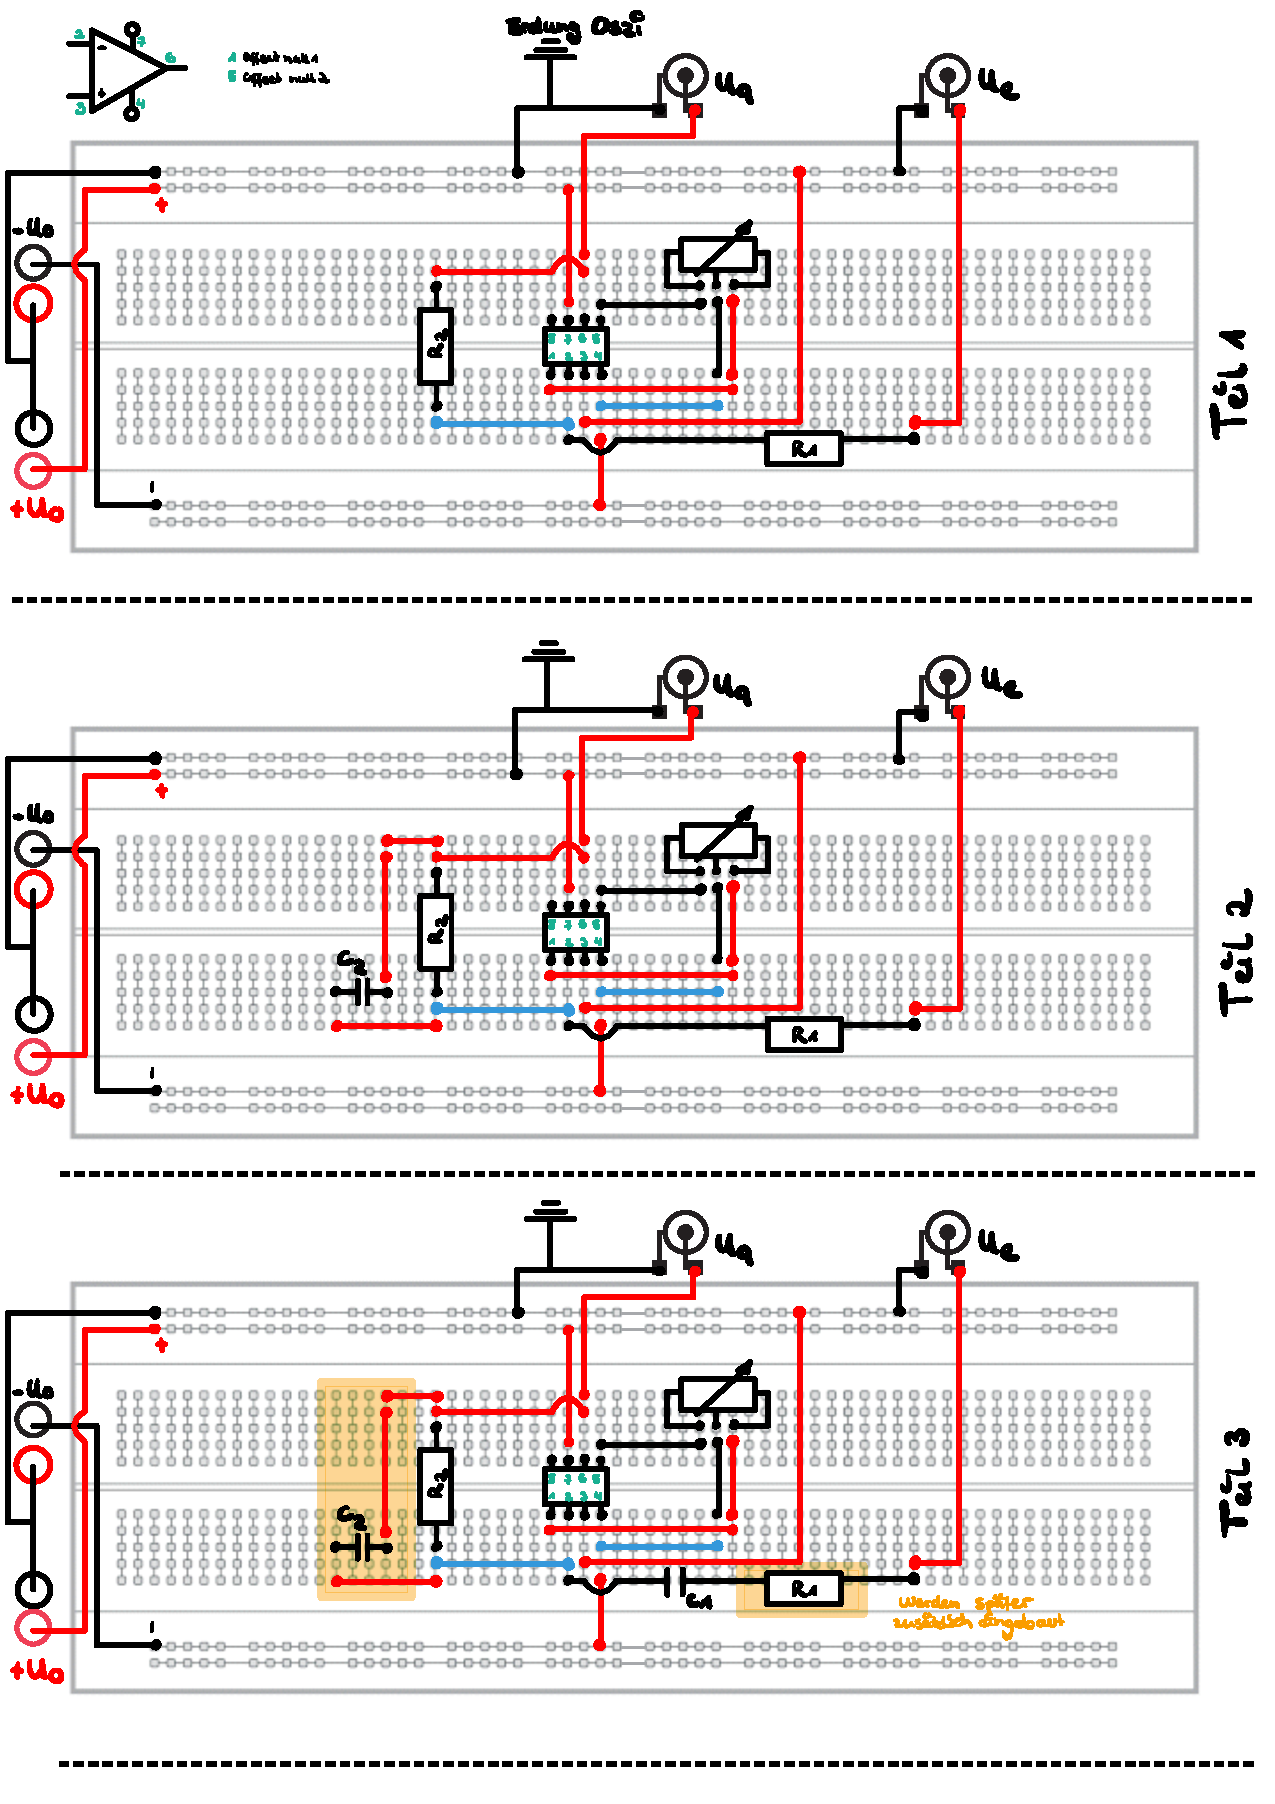
\includepdf[pages = -, landscape = false, nup = 1x1, scale = \skalierung , pagecommand={}]{30-SteckbretterEL2.pdf}
